% REV00 Tue 20 Jul 2021 08:12:01 WIB
% START Tue 20 Jul 2021 08:12:01 WIB

\chapter{Keempat}

% 11
\begin{figure}[htbp]
% h: here, where the figure appears in the text (use can always just use [h] )
% t: top,  top of the current page.
% b: bottom of the current page.
% p: page, top of the next available float space (sometimes end up being the end of the document).
\centerline{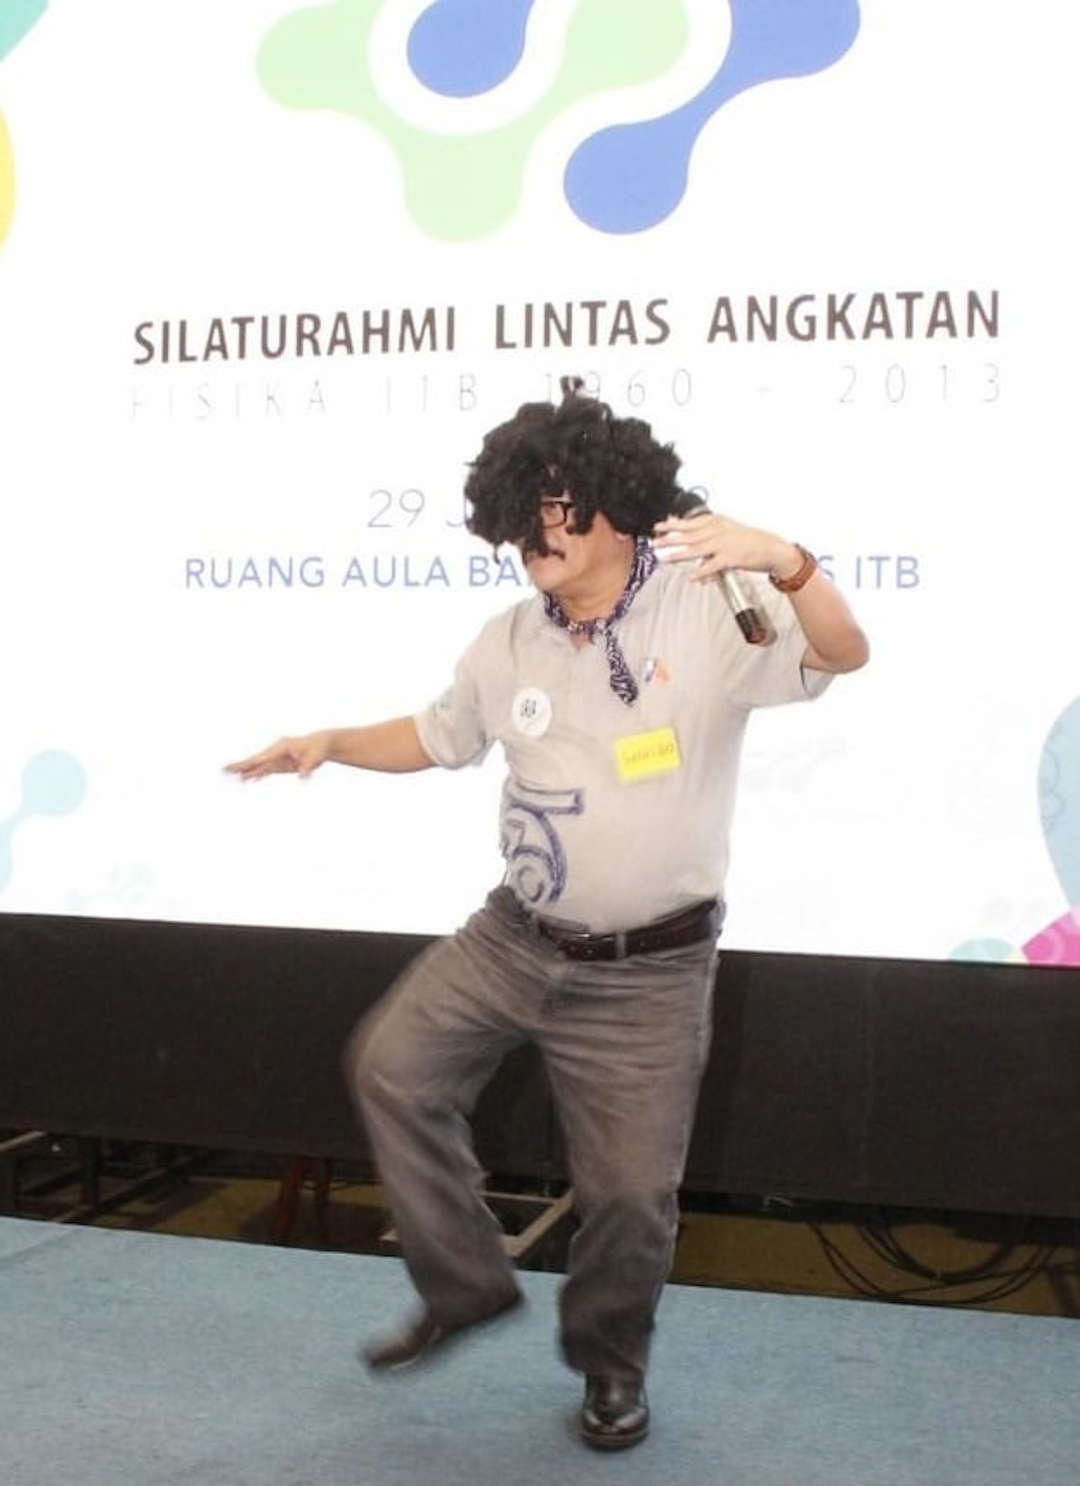
\includegraphics[scale=1.0]{01-04-01}}
\caption{ Roker/Dangduter Satiri dalam acara Reuni Alumni Fisika ITB 2018. Sumber: FB Satiri M Zen.}
\label{01-04-01}
\end{figure}
%

Walaupun dengan gontai, berangkat jugalah dia ke Bulungan. Satu-satunya alasan dia mau datang ke sana adalah karena sekolah itu dekat dengan tempat babanya berdagang kembang, di Jalan Melawai. Yang ia yakini cuma satu: Selepas sekolah ia bisa ikut dagang kembang. Yang lainnya, lihat situasi nanti sajalah.

Orang-orang bilang, kembang itu tidak akan berkompetisi dengan kembang lain walaupun dengan yang ada di sebelahnya. Mereka hanya berupaya berkembang saja.

Dengan persaingan yang super ketat, ia masih bisa berada di papan atas sekolah itu. Semester pertama dilaluinya dengan tertatih-tatih dalam biaya. Semester kedua dia memanfaatkan keraguannya itu dengan pengalaman kebaikan guru-gurunya waktu SMP. Datanglah ia menghadap Pak Lesilolo, sang legenda, Kepala Sekolah SMAN XI. Seperempat nadanya agak dinaikan, rada-rada mengancam:

“Pak, saya mau berhenti sekolah…”

“Lho, mengapa?”

“Saya tidak punya uang Pak…”

Maka terjadilah dialog atau tepatnya interogasi panjang, dengan keputusan akhir: Satiri harus terus sekolah, tidak boleh bolos, dan tidak perlu bayar uang sekolah!

Nah, Tuhan lagi-lagi menurunkan Gurunya yang ketiga. Maka Satiri pun semakin percaya diri. Tuhan yang tentunya memperhatikan kemampuan dan kemauan belajarnya.

Karena Satiri pintar dan gaul, ceplas-ceplos, kocak, kalau bicara cenderung seperti Lenong Betawi, maka teman-temannya sering mengundangnya ke rumah mereka untuk belajar bersama. Tepatnya, untuk santap siang sedap bergizi.

Suatu hari, selepas makan siang di rumah mewah salah seorang sahabatnya di bilangan Kebayoran Baru, Satiri dan kawan-kawannya itu belajar bersama di ruang terbuka lantai 2 menghadap ke muka rumah. Selepas belajar ketika sedang asik bercanda-ria, lewatlah babanya di depan rumah itu: babanya dengan sepeda onthel menjajakan bunga.

“Cublum cihuy…”, begitulah suara khas teriakan pedagang bunga keliling. Mungkin dari sepotong bahasa asing "bloem".

Satiri hanya bisa memandang babanya lewat dengan mulut menganga, diam sejuta bahasa, berasa ditampar popor senjata. Teman-temannya pun terkesima, aneh Satiri bisa diam seperti bata.

Fatherhood is the great thing that could ever happen. You can't explain it until it happens—it's like telling someone what water feels like before they've ever swam in it (Michael Bublé).

Bagaimanapun juga waktu terus berjalan. Satiri tetap di papan atas. Dari senior-seniornya pedagang kembang di Melawai dan Blok P (sekarang kantor Walikota Jakarta Selatan), dia juga belajar arti kehidupan, hal-hal baik maupun berbagai kenakalan: Warna sebenarnya dari hidup yang harus dihidupkan!

Kala itu, musik dangdut adalah penguasa musik nasional dengan raja bernama Rhoma Irama. Satiri tentu saja ikut joged di barisan paling depan. Saya teringat salah satu teriakan joged yang paling khas pada saat itu:

“Asiiikkk, ogah matiii… hooobah, ha… ha… ha…” (All right, don’t wanna die… yes, yes, yes…)

Sejak SMP dia belajar main gitar di jalanan, khususnya tentu buat dangdut. Kocokan gitar dan cengkok dangdut yg dimainkannya bagai menyatu dengan dirinya. Dia tidak pernah punya hambatan menyatakan dan mempromosikan selera musiknya. Menurutnya dangdut itu khas Indonesia, diciptakan dan dipopulerkan oleh orang Indonesia. Untuk itu adalah pantas dan wajib kalau kita bangga dengan dangdut. Jika orang Indonesia saja tidak suka, bagaimana mungkin mengharap orang lain untuk suka?

Buat Satiri, dangdut harus terus berjalan, ngaji juga tetap harus jalan. Di pertengahan SMA inilah Satiri berkenalan dengan Fitria, gadis mungil yang baru saja pindah ke Rawa Belong dan baru menginjak SMP. Fitria berasal dari keluarga Betawi yang cukup berada. Selain cantik, Betawi putih, Fitria juga pandai mengaji.

Jadilah mereka berdua pasangan juara musabaqoh tilawatil Qur’an se kelurahan.

Panjang gelombang alami mereka semakin berdekatan. Menurut Fisika Klasik, itu membangkitkan efek Doppler: saling memperkuatkan.

Menurut Fisika Kuantum, panjang gelombang menentukan realitas mereka di masa depan.

Ketika orang tua Fitria mengendus kedekatannya dengan Satiri, maka badai pun dimulai. Perbedaan status sosial.
\\[10pt]


Sumber tulisan asli \url{https://www.facebook.com/reno.alamsyah.94/posts/10226523934350700}

